\documentclass[12pt]{beamer}
\usetheme{metropolis}
\newenvironment{code}{\ttfamily}{\par}
\title{Where does \textit{your} compiler come from?}
\date{2018-03-13}
\author{Vincent Ambo}
\institute{Norwegian Unix User Group}
\begin{document}
  \maketitle

  %% Slide 1:
  \section{Introduction}

  %% Slide 2:
  \begin{frame}{Chicken and egg}
    Self-hosted compilers are often built using themselves, for example:

    \begin{itemize}
    \item C-family compilers bootstrap themselves \& each other
    \item (Some!) Common Lisp compilers can bootstrap each other
    \item \texttt{rustc} bootstraps itself with a previous version
    \item ... same for many other languages!
    \end{itemize}
  \end{frame}

  %% Slide 3:
  \begin{frame}{Trusting Trust}
    \begin{center}
      \huge{Could this be exploited?}
    \end{center}
  \end{frame}

  %% Slide 4:
  \begin{frame}{Short interlude: A quine}
    \begin{center}
      \begin{code}
        ((lambda (x) (list x (list 'quote x)))
        \newline\vspace*{6mm} '(lambda (x) (list x (list 'quote x))))
      \end{code}
    \end{center}
  \end{frame}

  %% Slide 5:
  \begin{frame}{Short interlude: Quine Relay}
    \begin{center}
      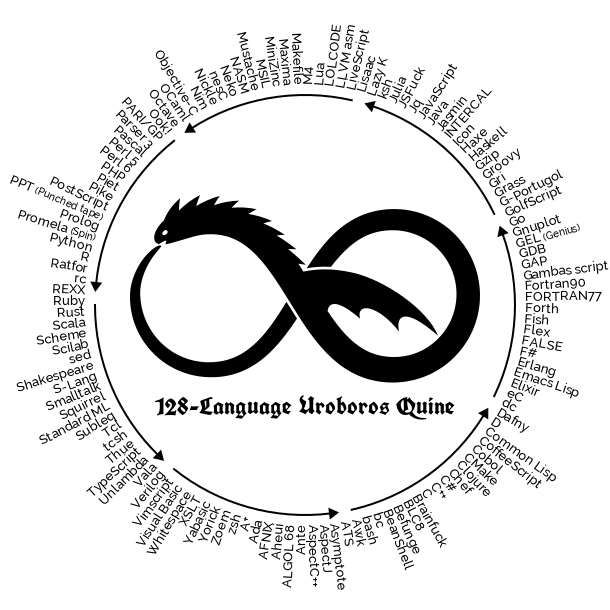
\includegraphics[
        keepaspectratio=true,
        height=\textheight
      ]{quine-relay.png}
    \end{center}
  \end{frame}

  %% Slide 6:
  \begin{frame}{Trusting Trust}
    An attack described by Ken Thompson in 1983:

    \begin{enumerate}
    \item Modify a compiler to detect when it's compiling itself.
    \item Let the modification insert \textit{itself} into the new compiler.
    \item Add arbitrary attack code to the modification.
    \item \textit{Optional!} Remove the attack from the source after compilation.
    \end{enumerate}
  \end{frame}

  %% Slide 7:
  \begin{frame}{Damage potential?}
    \begin{center}
      \large{Let your imagination run wild!}
    \end{center}
  \end{frame}

  %% Slide 8:
  \section{Countermeasures}

  %% Slide 9:
  \begin{frame}{Diverse Double-Compiling}
    Assume we have:

    \begin{itemize}
    \item Target language compilers $A$ and $T$
    \item The source code of $A$: $ S_{A} $
    \end{itemize}
  \end{frame}

  %% Slide 10:
  \begin{frame}{Diverse Double-Compiling}
    Apply the first stage (functional equivalence):

    \begin{itemize}
    \item $ X = A(S_{A})$
    \item $ Y = T(S_{A})$
    \end{itemize}

    Apply the second stage (bit-for-bit equivalence):

    \begin{itemize}
    \item $ V = X(S_{A})$
    \item $ W = Y(S_{A})$
    \end{itemize}

    Now we have a new problem: Reproducibility!
  \end{frame}

  %% Slide 11:
  \begin{frame}{Reproducibility}
    Bit-for-bit equivalent output is hard, for example:

    \begin{itemize}
    \item Timestamps in output artifacts
    \item Non-deterministic linking order in concurrent builds
    \item Non-deterministic VM \& memory states in outputs
    \item Randomness in builds (sic!)
    \end{itemize}
  \end{frame}

  \begin{frame}{Reproducibility}
    \begin{center}
      Without reproducibility, we can never trust that any shipped
      binary matches the source code!
    \end{center}
  \end{frame}

  %% Slide 12:
  \section{(Partial) State of the Union}

  \begin{frame}{The Desired State}
    \begin{center}
      \begin{enumerate}
      \item Full-source bootstrap!
      \item All packages reproducible!
      \end{enumerate}
    \end{center}
  \end{frame}

  %% Slide 13:
  \begin{frame}{Bootstrapping Debian}
    \begin{itemize}
    \item Sparse information on the Debian-wiki
    \item Bootstrapping discussions mostly resolve around new architectures
    \item GCC is compiled by depending on previous versions of GCC
    \end{itemize}
  \end{frame}

  \begin{frame}{Reproducing Debian}
    Debian has a very active effort for reproducible builds:

    \begin{itemize}
    \item Organised information about reproducibility status
    \item Over 90\% reproducibility in Debian package base!
    \end{itemize}
  \end{frame}

  \begin{frame}{Short interlude: Nix}
    \begin{center}
      
\includegraphics[
        keepaspectratio=true,
        height=0.7\textheight
      ]{nixos-logo.png}
    \end{center}
  \end{frame}

  \begin{frame}{Short interlude: Nix}
    \begin{center}
      
\includegraphics[
        keepaspectratio=true,
        height=0.90\textheight
      ]{drake-meme.png}
    \end{center}
  \end{frame}

  \begin{frame}{Short interlude: Nix}
    \begin{center}
      
\includegraphics[
        keepaspectratio=true,
        height=0.7\textheight
      ]{nixos-logo.png}
    \end{center}
  \end{frame}

  \begin{frame}{Bootstrapping NixOS}
    Nix evaluation can not recurse forever: The bootstrap can not
    simply depend on a previous GCC.

    Result: \texttt{bootstrap-tools} tarball from a previous binary
    cache is fetched and used.

    An unfortunate magic binary blob ...
  \end{frame}

  \begin{frame}{Reproducing NixOS}
    Not all reproducibility patches have been ported from Debian.

    However: Builds are fully repeatable via the Nix fundamentals!
  \end{frame}

  \section{Future Developments}

  \begin{frame}{Bootstrappable: stage0}
    Hand-rolled ``Cthulhu's Path to Madness'' hex-programs:

    \begin{itemize}
    \item No non-auditable binary blobs
    \item Aims for understandability by 70\% of programmers
    \item End goal is a full-source bootstrap of GCC
    \end{itemize}
  \end{frame}


  \begin{frame}{Bootstrappable: MES}
    Bootstrapping the ``Maxwell Equations of Software'':

    \begin{itemize}
    \item Minimal C-compiler written in Scheme
    \item Minimal Scheme-interpreter (currently in C, but intended to
      be rewritten in stage0 macros)
    \item End goal is full-source bootstrap of the entire GuixSD
    \end{itemize}
  \end{frame}

  \begin{frame}{Other platforms}
    \begin{itemize}
    \item Nix for Darwin is actively maintained
    \item F-Droid Android repository works towards fully reproducible
      builds of (open) Android software
    \item Mobile devices (phones, tablets, etc.) are a lost cause at
      the moment
    \end{itemize}
  \end{frame}

  \begin{frame}{Thanks!}
    Resources:
    \begin{itemize}
    \item bootstrappable.org
    \item reproducible-builds.org
    \end{itemize}

    @tazjin | mail@tazj.in
  \end{frame}
\end{document}
